\documentclass[oneside,12pt]{article}
\usepackage{indentfirst}
\usepackage{fullpage}
\usepackage{blindtext, graphicx}
\usepackage{graphicx}
\usepackage[toc,page]{appendix}
\usepackage{lipsum}
\usepackage{booktabs}
\usepackage{caption}
\usepackage{tabularx}
\usepackage{amsmath}
\usepackage{gensymb}
\usepackage{tabu}
\usepackage{float}
\usepackage{url}
\usepackage{subfigure}
%\usepackage{listings}
\usepackage[framed,numbered]{matlab-prettifier}
\usepackage{color}
\usepackage[colorlinks=true,linkcolor=black, urlcolor=blue]{hyperref}
\setlength{\tabcolsep}{20pt}





\begin{document}

\tableofcontents
\newpage
\section{Introduction}

\begin{figure}[H]
	\centering
	\includegraphics[width=11cm, height=10cm]{"Buck Boost Simulink Model"}
	\caption{ Buck Boost Simulink Model}
	\label{fig:buck-boost-simulink-model}
\end{figure}


\section{Question 1}


\begin{figure}[H]
	\centering
	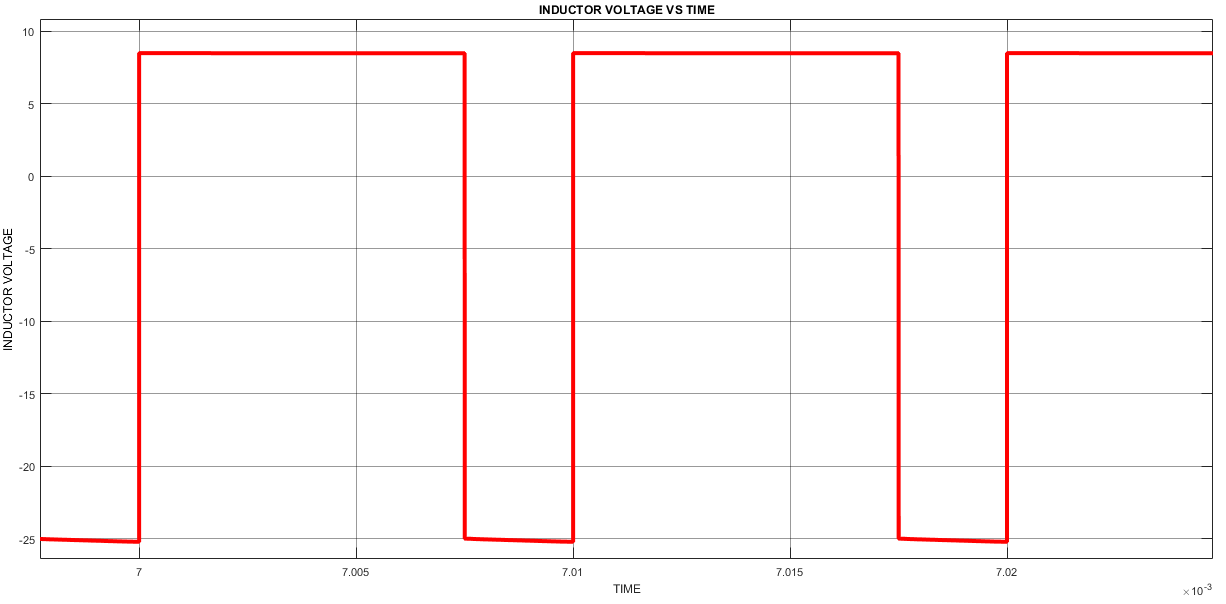
\includegraphics[width=14cm, height=8cm]{q1/V_L}
	\caption{Inductor Voltage}
	\label{fig:vl}
\end{figure}
\begin{figure}[H]
	\centering
	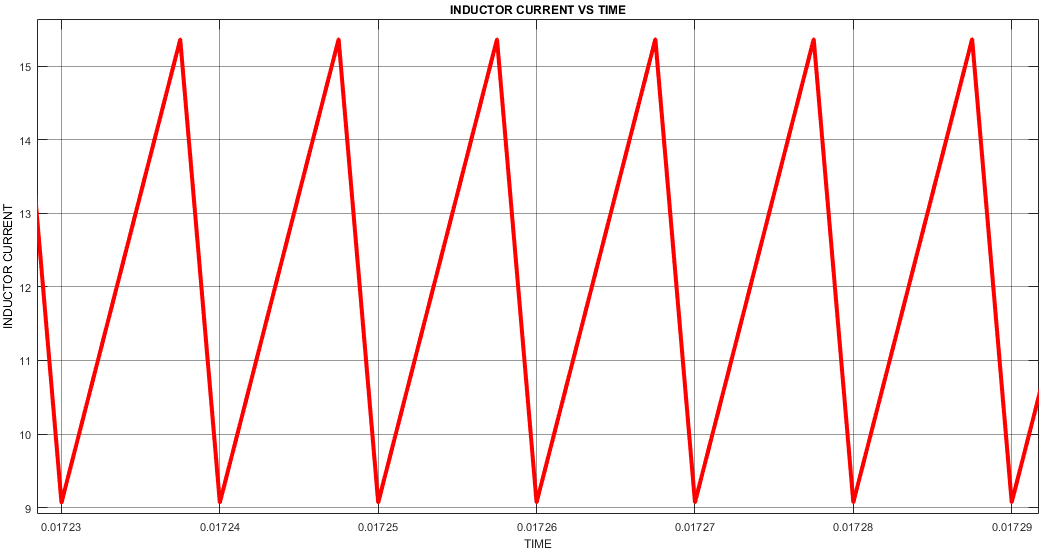
\includegraphics[width=14cm, height=8cm]{q1/I_L}
	\caption{Inductor Current}
	\label{fig:il}
\end{figure}
\begin{figure}[H]
	\centering
	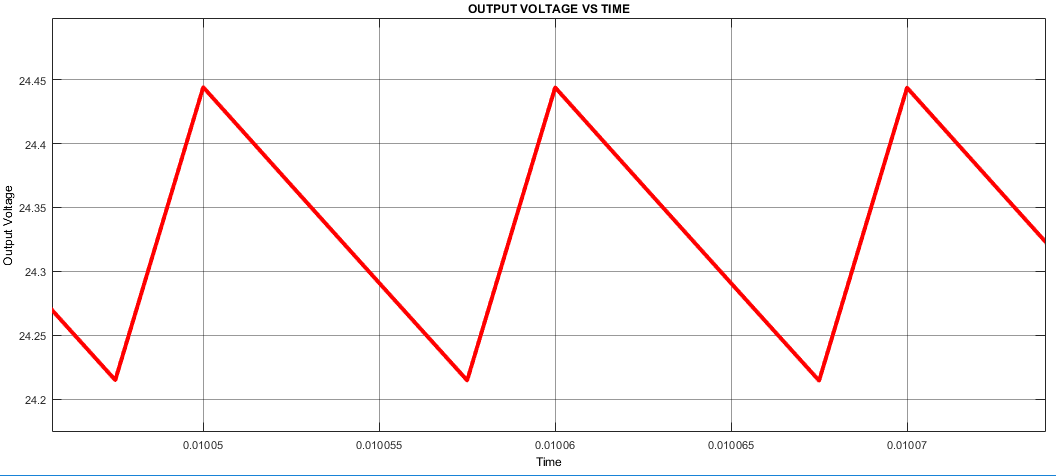
\includegraphics[width=14cm, height=8cm]{q1/vout}
	\caption{Output Voltage}
	\label{fig:vout}
\end{figure}
\begin{figure}[H]
	\centering
	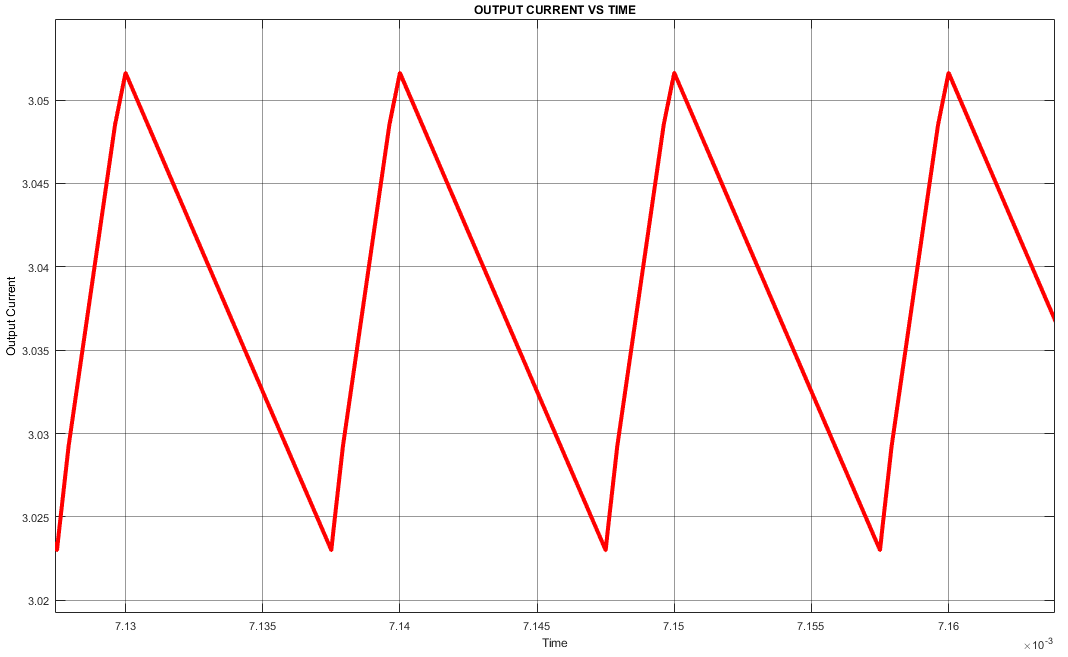
\includegraphics[width=14cm, height=8cm]{q1/Iout}
	\caption{Output Current}
	\label{fig:iout}
\end{figure}
\begin{figure}[H]
	\centering
	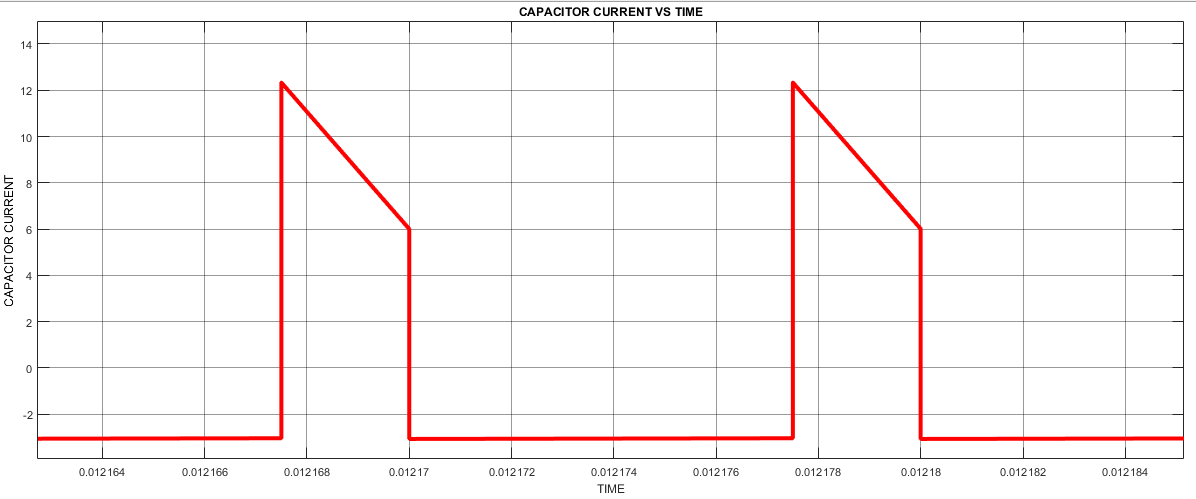
\includegraphics[width=14cm, height=8cm]{q1/I_CAP}
	\caption{Capacitor Current}
	\label{fig:icap}
\end{figure}


\newpage
\section{Question 2}
\begin{figure}[H]
	\centering
	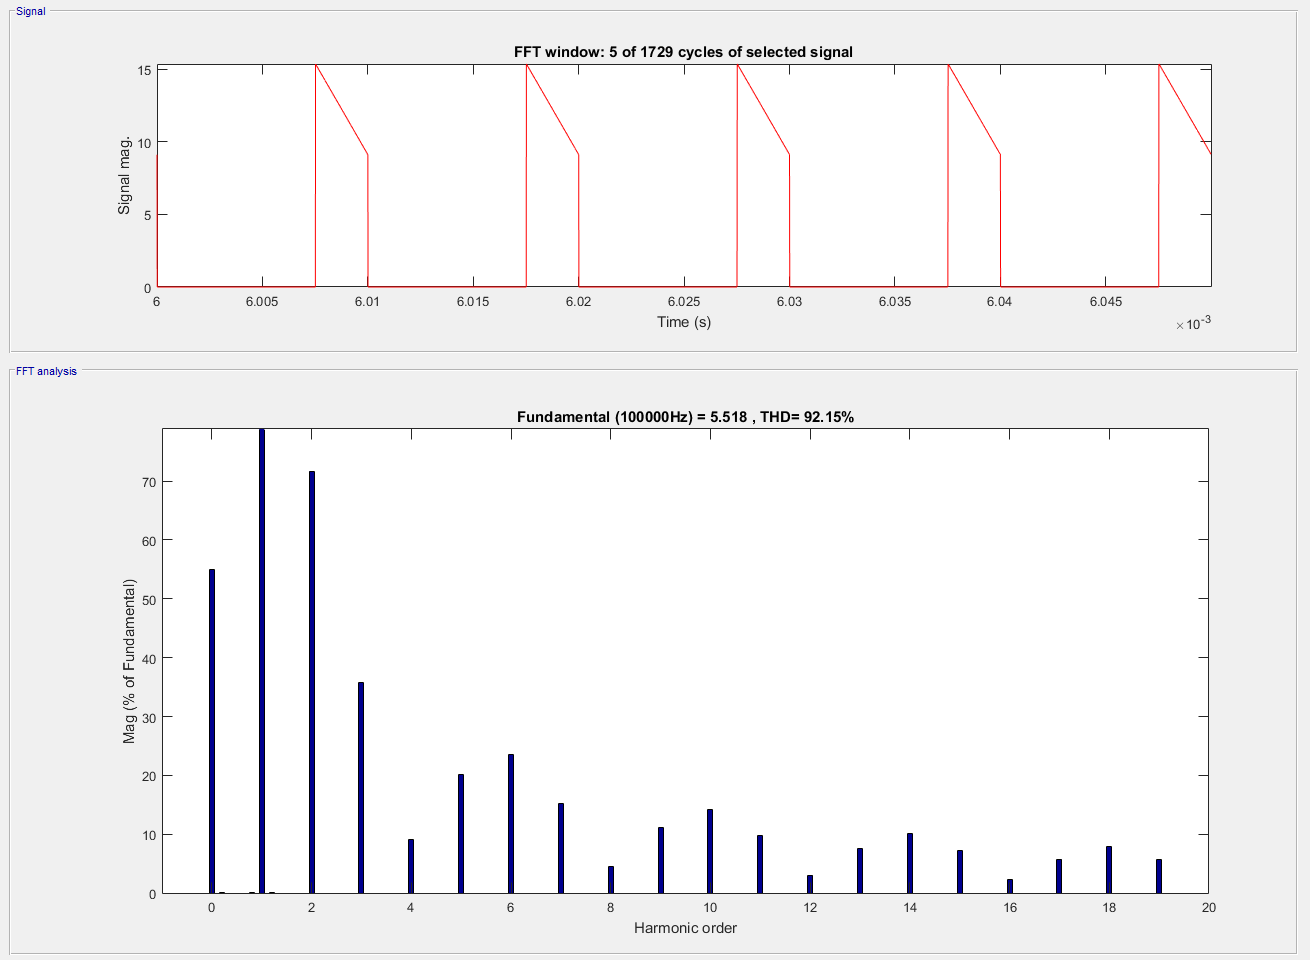
\includegraphics[width=14cm, height=8cm]{q2/HarmonikFFT}
	\caption{Diode Currents FFT Analysis}
	\label{fig:harmonikfft}
\end{figure}
THD is found to be \%94.


\newpage\section{Question 3}

\begin{figure}[H]
	\centering
	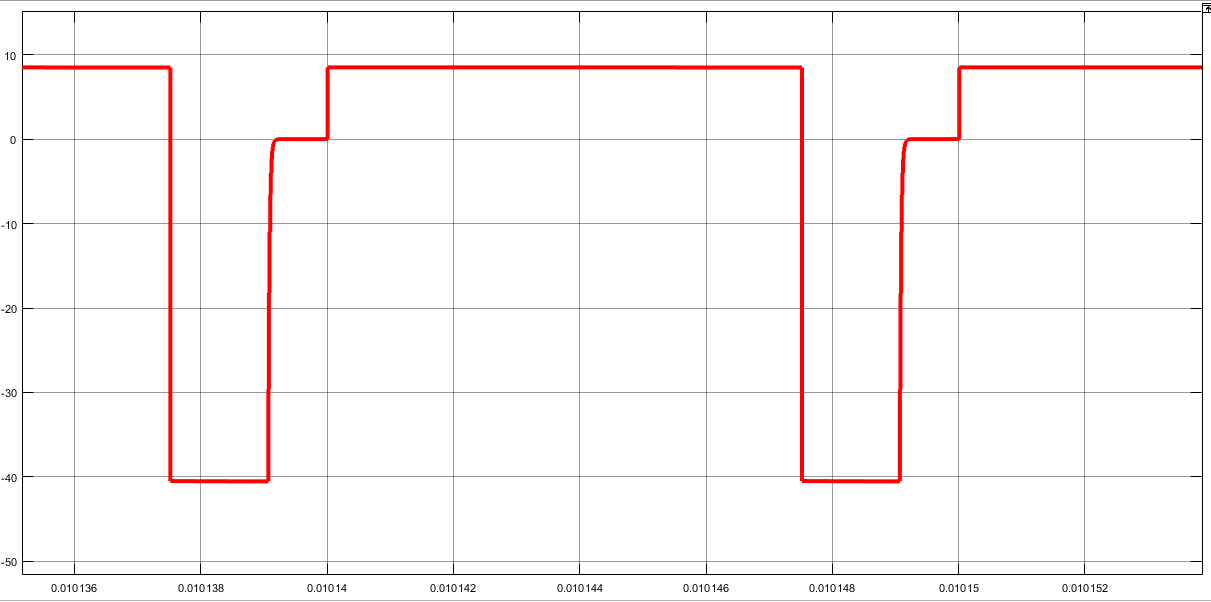
\includegraphics[scale=0.5]{q3/VL}
	\caption{DCM Inductor Voltage Waveform}
	\label{fig:vl}
\end{figure}
\begin{figure}[H]
	\centering
	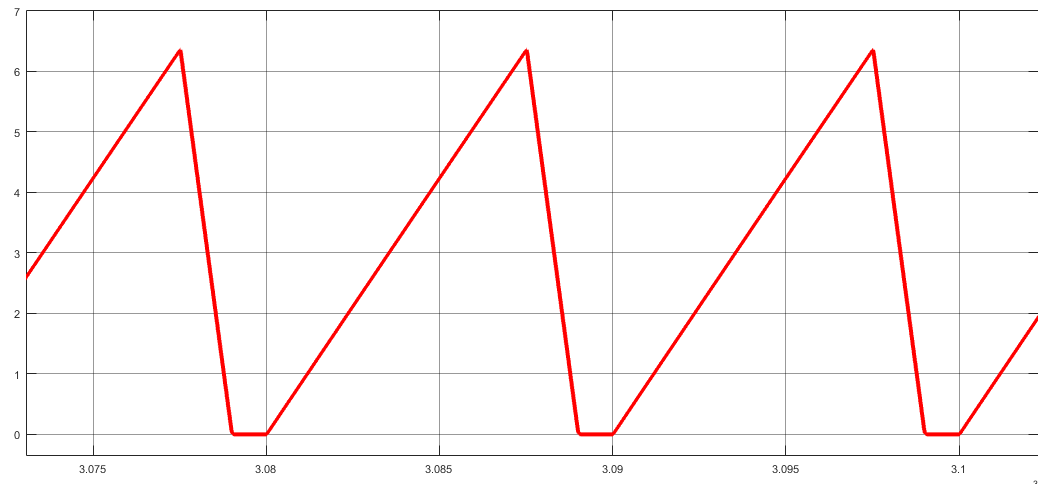
\includegraphics[scale=0.5]{q3/IL}
	\caption{DCM Inductor Current Waveform}
	\label{fig:il}
\end{figure}


\newpage\section{Question 4}

\begin{figure}[H]
	\centering
	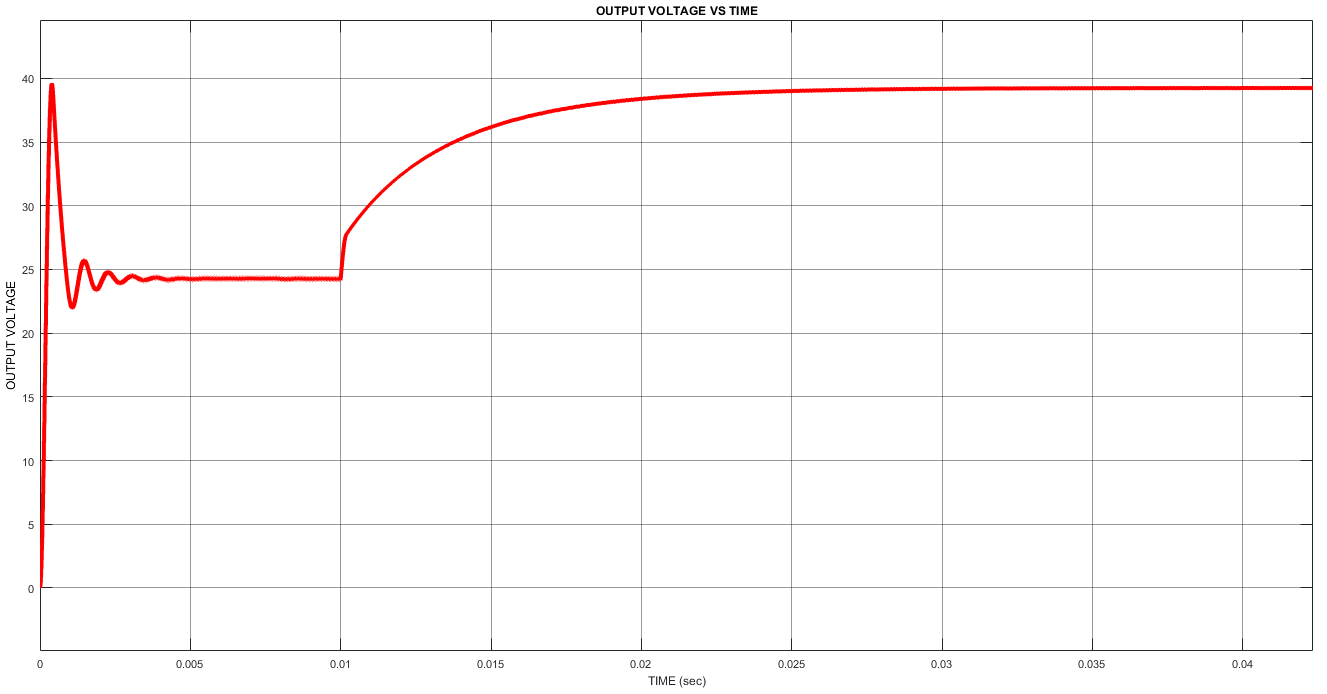
\includegraphics[width=14cm, height=8cm]{Q4/yeni/VOUT}
	\caption{CCM to DCM Output Voltage (Open Loop Operation)}
	\label{fig:vout}
\end{figure}
\begin{figure}[H]
	\centering
	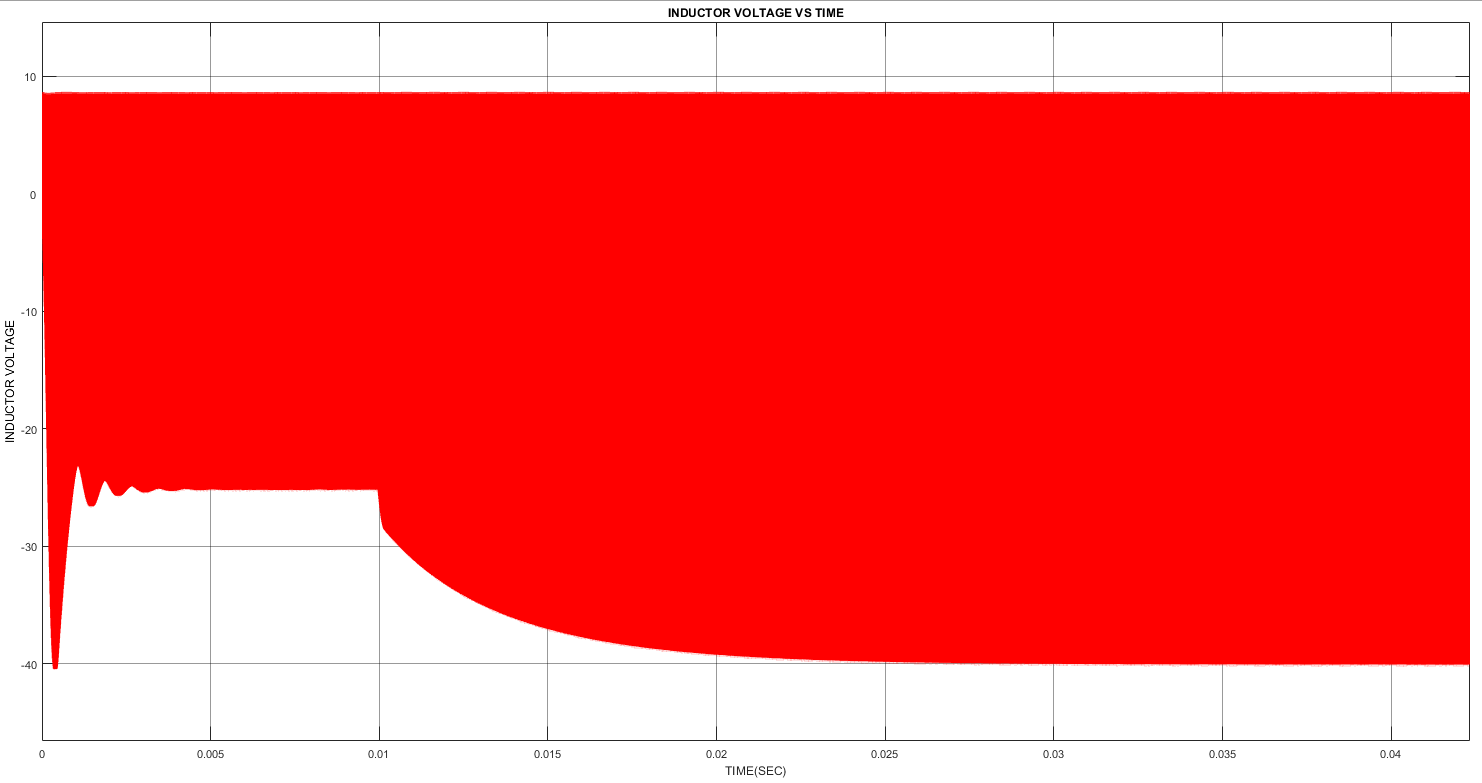
\includegraphics[width=14cm, height=8cm]{Q4/yeni/VL}
	\caption{CCM to DCM Inductor Voltage (Open Loop Operation)}
	\label{fig:vl}
\end{figure}
\begin{figure}[H]
	\centering
	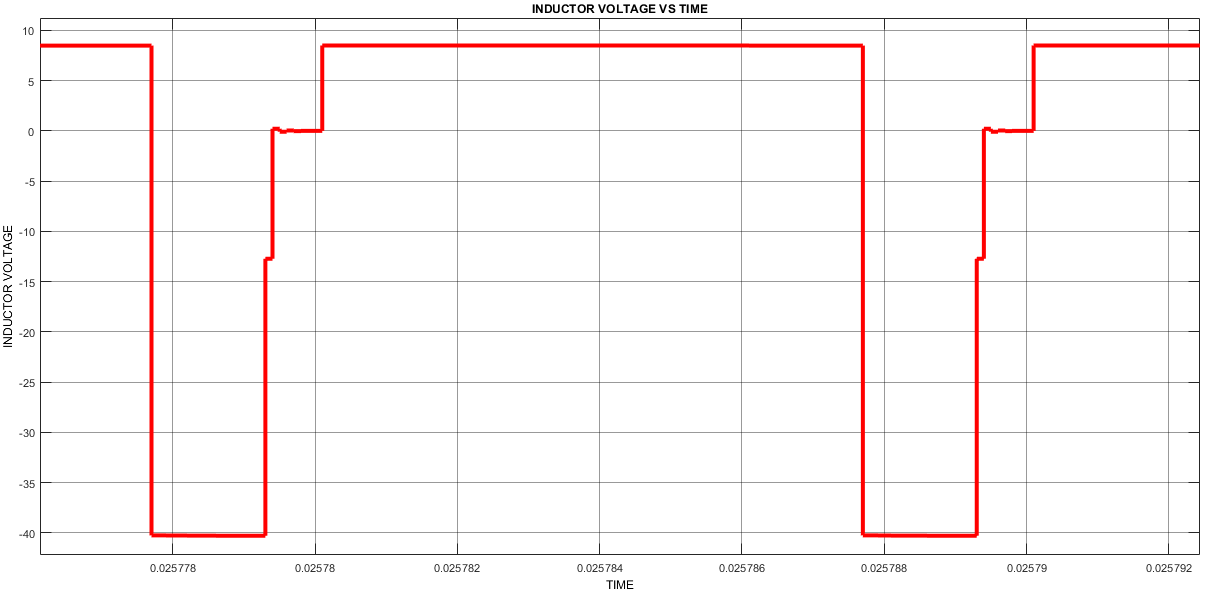
\includegraphics[width=14cm, height=8cm]{Q4/yeni/VLzoom}
	\caption{CCM to DCM Inductor Voltage Zoomed (Open Loop Operation)}
	\label{fig:vlzoom}
\end{figure}
\begin{figure}[H]
	\centering
	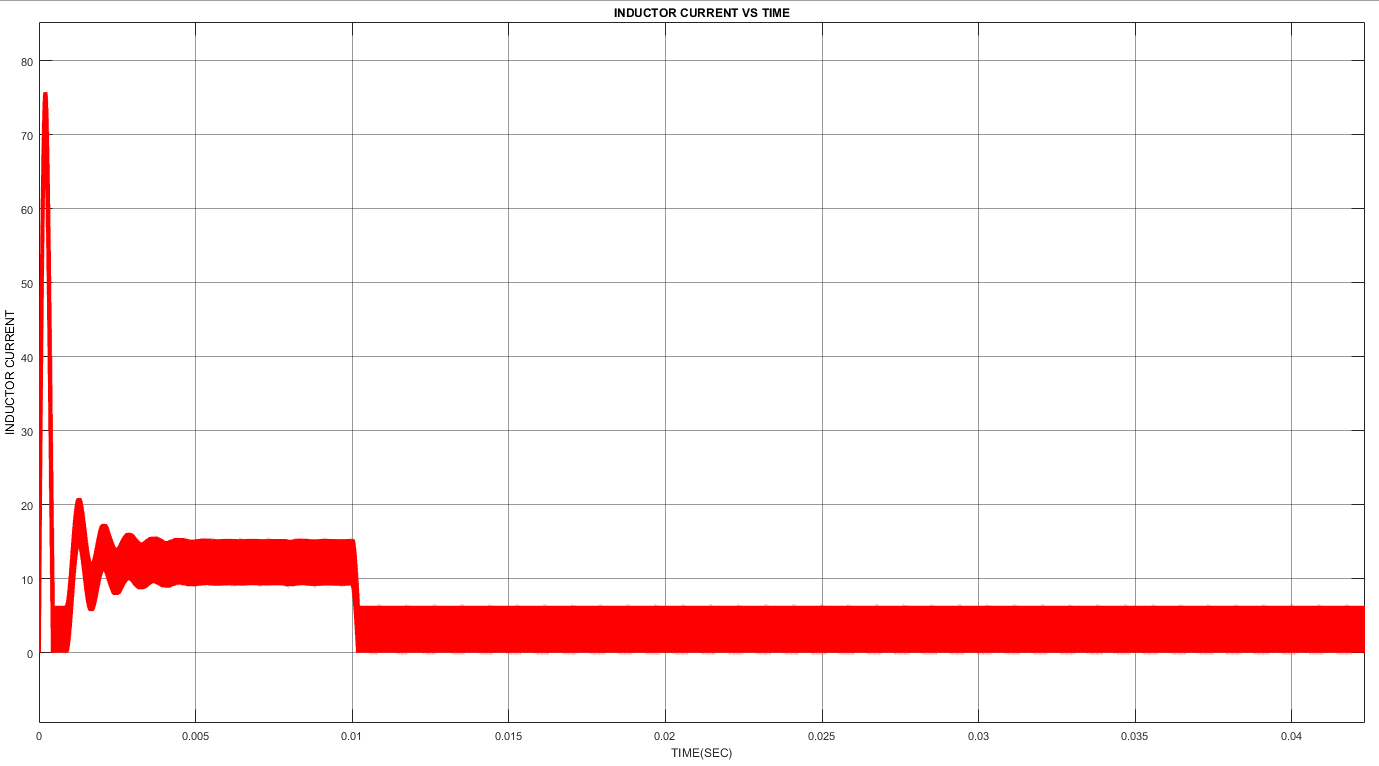
\includegraphics[width=14cm, height=8cm]{Q4/yeni/IL}
	\caption{CCM to DCM Inductor Current (Open Loop Operation)}
	\label{fig:il}
\end{figure}
\begin{figure}[H]
	\centering
	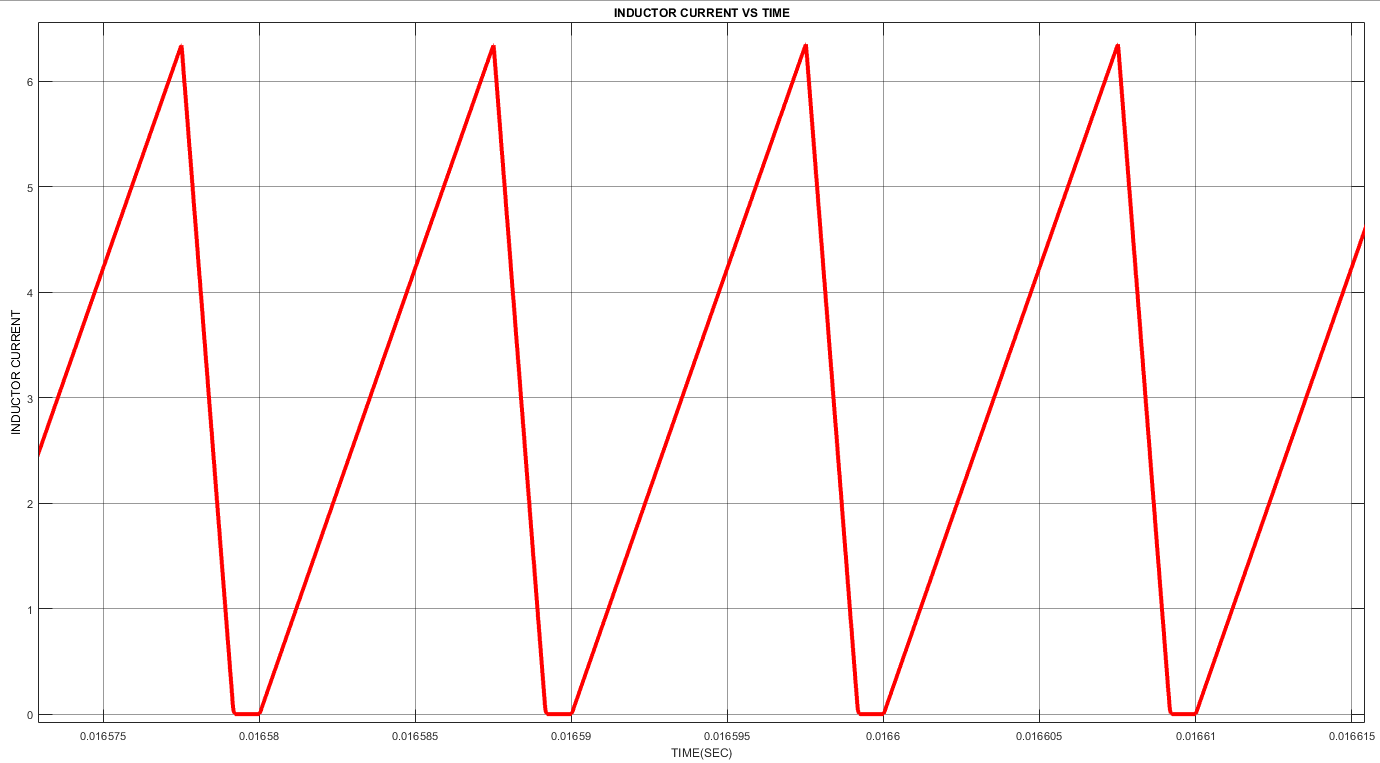
\includegraphics[width=14cm, height=8cm]{Q4/yeni/ILZOOM_DCM}
	\caption{CCM to DCM Inductor Current Zoomed(Open Loop Operation)}
	\label{fig:ilzoomdcm}
\end{figure}




\newpage\section{Question 5}

\begin{figure}[H]
	\centering
	\includegraphics[width=14cm, height=8cm]{"q5/peak to peak output voltage"}
	\caption{Output Voltage in Steady State}
	\label{fig:peak-to-peak-output-voltage}
\end{figure}

\begin{figure}[H]
	\centering
	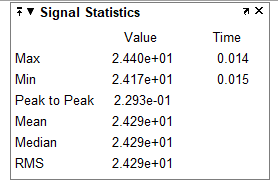
\includegraphics[width=14cm, height=8cm]{q5/statistics}
	\caption{Waveform information of Output Voltage in Steady State}
	\label{fig:statistics}
\end{figure}


\newpage\section{Question 6}



\begin{figure}[H]
	\centering
	\includegraphics[width=6cm, height=3cm]{"q6/rmscalc"}
	\caption{RMS calculation of Capacitor Current in CCM }
	\label{fig:ekran-alnts}
\end{figure}



\end{document}